% answers.tex —— 2007 年·全国大纲卷Ⅰ·文科 · 参考答案与详细解析片段
% 由 tools/generate_projects.py 依来源总账自 2007/2007_数学真题_全国1文_试题.md + 2007/2007_数学真题_全国1文_解析正文.md + 2007/2007_数学真题_全国1文_答案要点.md 生成，勿手改（改源 MD 后重跑）


\begin{gktip}
固定源 PDF 为印刷页码 361–362 的两页题面，不附答案。以下解析均依据固定源独立复算；第 7、19 题图形在 LaTeX 工程中以 TikZ/PGFPlots 矢量源重绘。
\end{gktip}

\begin{answer}
\gksolhead{1}{}

\textbf{题目}：

设 $S=\{x\mid2x+1>0\}$，$T=\{x\mid3x-5<0\}$，则 $S\cap T=$\mbox{（　　）}

（A）$\varnothing$\quad（B）$\{x\mid x<-\dfrac12\}$\quad（C）$\{x\mid x>\dfrac53\}$\quad（D）$\{x\mid-\dfrac12<x<\dfrac53\}$

\Needspace{4\baselineskip}
\textbf{解析}

由 $2x+1>0$ 得 $x>-\dfrac12$，由 $3x-5<0$ 得 $x<\dfrac53$，交集为 $\left(-\dfrac12,\dfrac53\right)$。

\gkanswer{答案：D}

\end{answer}
\begin{answer}
\gksolhead{2}{}

\textbf{题目}：

$\alpha$ 是第四象限角，$\cos\alpha=\dfrac{12}{13}$，则 $\sin\alpha=$\mbox{（　　）}

（A）$\dfrac5{13}$\quad（B）$-\dfrac5{13}$\quad（C）$\dfrac5{12}$\quad（D）$-\dfrac5{12}$

\Needspace{4\baselineskip}
\textbf{解析}

\Needspace{5\baselineskip}
第四象限角的正弦为负，且

\nopagebreak[4]
\[
\sin\alpha=-\sqrt{1-\cos^2\alpha}=-\frac5{13}
\]
。

\gkanswer{答案：B}

\end{answer}
\begin{answer}
\gksolhead{3}{}

\textbf{题目}：

已知向量 $\boldsymbol a=(-5,6)$，$\boldsymbol b=(6,5)$，则 $\boldsymbol a$ 与 $\boldsymbol b$\mbox{（　　）}

（A）垂直\quad（B）不垂直也不平行\quad（C）平行且同向\quad（D）平行且反向

\Needspace{4\baselineskip}
\textbf{解析}

\nopagebreak[4]
\[
\boldsymbol a\cdot\boldsymbol b=(-5)6+6\cdot5=0
\]
，

所以两向量垂直。

\gkanswer{答案：A}

\end{answer}
\begin{answer}
\gksolhead{4}{}

\textbf{题目}：

已知双曲线的离心率为 $2$，焦点是 $(-4,0),(4,0)$，则双曲线方程为\mbox{（　　）}

（A）$\dfrac{x^2}{4}-\dfrac{y^2}{12}=1$\quad（B）$\dfrac{x^2}{12}-\dfrac{y^2}{4}=1$\quad（C）$\dfrac{x^2}{10}-\dfrac{y^2}{6}=1$\quad（D）$\dfrac{x^2}{6}-\dfrac{y^2}{10}=1$

\Needspace{4\baselineskip}
\textbf{解析}

\Needspace{5\baselineskip}
焦半距 $c=4$，离心率 $e=2$，故 $a=c/e=2$，并且 $b^2=c^2-a^2=12$，方程为

\nopagebreak[4]
\[
\frac{x^2}{4}-\frac{y^2}{12}=1
\]
。

\gkanswer{答案：A}

\end{answer}
\begin{answer}
\gksolhead{5}{}

\textbf{题目}：

甲、乙、丙 $3$ 位同学选修课程，从 $4$ 门课程中，甲选修 $2$ 门，乙、丙各选修 $3$ 门，则不同的选修方案共有\mbox{（　　）}

（A）$36$ 种\quad（B）$48$ 种\quad（C）$96$ 种\quad（D）$192$ 种

\Needspace{4\baselineskip}
\textbf{解析}

\Needspace{5\baselineskip}
三位同学的选课方案彼此独立，方案数为

\nopagebreak[4]
\[
\binom42\binom43\binom43=6\cdot4\cdot4=96
\]
。

\gkanswer{答案：C}

\end{answer}
\begin{answer}
\gksolhead{6}{}

\textbf{题目}：

\Needspace{5\baselineskip}
下面给出的四个点中，位于不等式组

\nopagebreak[4]
\[
\begin{cases}
x+y-1<0,\\
x-y+1>0
\end{cases}
\]

表示的平面区域内的点是\mbox{（　　）}

（A）$(0,2)$\quad（B）$(-2,0)$\quad（C）$(0,-2)$\quad（D）$(2,0)$

\Needspace{4\baselineskip}
\textbf{解析}

逐点代入可行域。点 $(0,-2)$ 满足 $x+y-1<0$ 且 $x-y+1>0$，其余三点至少违反一个不等式。

\gkanswer{答案：C}

\end{answer}
\begin{answer}
\gksolhead{7}{}

\textbf{题目}：

如图，正四棱柱 $ABCD-A_1B_1C_1D_1$ 中，$AA_1=2AB$，则异面直线 $A_1B$ 与 $AD_1$ 所成角的余弦值为\mbox{（　　）}
\nopagebreak[4]
\begin{center}% 2007 年全国大纲卷Ⅰ文科第 7 题：正四棱柱
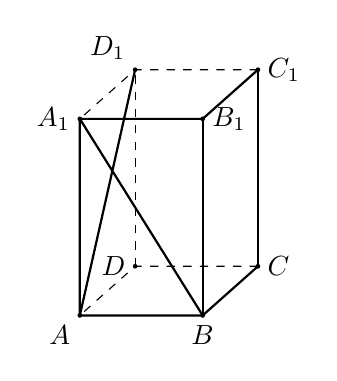
\begin{tikzpicture}[>=stealth,scale=0.78]
  \coordinate (A) at (0,0); \coordinate (B) at (2.0,0);
  \coordinate (C) at (2.9,0.8); \coordinate (D) at (0.9,0.8);
  \coordinate (A1) at (0,3.2); \coordinate (B1) at (2,3.2);
  \coordinate (C1) at (2.9,4.0); \coordinate (D1) at (0.9,4.0);
  \draw[thick] (A)--(B)--(C); \draw[dashed] (C)--(D)--(A);
  \draw[thick] (A)--(A1)--(B1)--(C1);
  \draw[dashed] (C1)--(D1)--(A1);
  \draw[thick] (B)--(B1) (C)--(C1);
  \draw[dashed] (D)--(D1);
  \draw[thick] (A1)--(B) (A)--(D1);
  \fill (A) circle (1.1pt) node[below left] {$A$};
  \fill (B) circle (1.1pt) node[below] {$B$};
  \fill (C) circle (1.1pt) node[right] {$C$};
  \fill (D) circle (1.1pt) node[left] {$D$};
  \fill (A1) circle (1.1pt) node[left] {$A_1$};
  \fill (B1) circle (1.1pt) node[right] {$B_1$};
  \fill (C1) circle (1.1pt) node[right] {$C_1$};
  \fill (D1) circle (1.1pt) node[above left] {$D_1$};
\end{tikzpicture}
\end{center}
\nopagebreak[4]
（A）$\dfrac15$\quad（B）$\dfrac25$\quad（C）$\dfrac35$\quad（D）$\dfrac45$

\Needspace{4\baselineskip}
\textbf{解析}

\Needspace{5\baselineskip}
令 $AB=1,AA_1=2$，取

\nopagebreak[4]
\[
A=(0,0,0),\ B=(1,0,0),\ D=(0,1,0),\ A_1=(0,0,2),\ D_1=(0,1,2)
\]
。

\Needspace{5\baselineskip}
则

\nopagebreak[4]
\[
\overrightarrow{A_1B}=(1,0,-2),\qquad
\overrightarrow{AD_1}=(0,1,2),
\]

两向量内积为 $-4$，长度均为 $\sqrt5$，故异面直线的锐角夹角余弦为 $\dfrac45$。

\gkanswer{答案：D}

\end{answer}
\begin{answer}
\gksolhead{8}{}

\textbf{题目}：

设 $a>1$，函数 $f(x)=\log_a x$ 在区间 $[a,2a]$ 上的最大值与最小值之差为 $\dfrac12$，则 $a=$\mbox{（　　）}

（A）$\sqrt2$\quad（B）$2$\quad（C）$2\sqrt2$\quad（D）$4$

\Needspace{4\baselineskip}
\textbf{解析}

\Needspace{5\baselineskip}
因 $a>1$，$f$ 在 $[a,2a]$ 上递增，最大值与最小值之差为

\nopagebreak[4]
\[
\log_a(2a)-\log_a a=\log_a2=\frac12
\]
，

所以 $a=4$。

\gkanswer{答案：D}

\end{answer}
\begin{answer}
\gksolhead{9}{}

\textbf{题目}：

$f(x),g(x)$ 是定义在 $\mathbb R$ 上的函数，$h(x)=f(x)+g(x)$，则“$f(x),g(x)$ 均为偶函数”是“$h(x)$ 为偶函数”的\mbox{（　　）}

（A）充要条件\quad（B）充分而不必要的条件\quad（C）必要而不充分的条件\quad（D）既不充分也不必要的条件

\Needspace{4\baselineskip}
\textbf{解析}

若 $f,g$ 均为偶函数，则 $h=f+g$ 必为偶函数；反之取 $f(x)=x,g(x)=-x$，则 $h$ 为偶函数而 $f,g$ 都不是偶函数。因此这是充分而不必要条件。

\gkanswer{答案：B}

\end{answer}
\begin{answer}
\gksolhead{10}{}

\textbf{题目}：

函数 $y=2\cos^2x$ 的一个单调增区间是\mbox{（　　）}

（A）$\left(-\dfrac\pi4,\dfrac\pi4\right)$\quad（B）$\left(0,\dfrac\pi2\right)$\quad（C）$\left(\dfrac\pi4,\dfrac{3\pi}4\right)$\quad（D）$\left(\dfrac\pi2,\pi\right)$

\Needspace{4\baselineskip}
\textbf{解析}

\nopagebreak[4]
\[
2\cos^2x=1+\cos2x,\qquad
f'(x)=-2\sin2x
\]
。

在 $\left(\dfrac\pi2,\pi\right)$ 内 $\sin2x<0$，故函数递增。

\gkanswer{答案：D}

\end{answer}
\begin{answer}
\gksolhead{11}{}

\textbf{题目}：

曲线 $y=\dfrac13x^3+x$ 在点 $\left(1,\dfrac43\right)$ 处的切线与坐标轴围成的三角形面积为\mbox{（　　）}

（A）$\dfrac19$\quad（B）$\dfrac29$\quad（C）$\dfrac13$\quad（D）$\dfrac23$

\Needspace{4\baselineskip}
\textbf{解析}

\Needspace{5\baselineskip}
切线斜率为 $x^2+1$，在 $x=1$ 处为 $2$，切线为

\nopagebreak[4]
\[
y-\frac43=2(x-1)\Longrightarrow y=2x-\frac23
\]
。

与坐标轴截距的绝对值为 $\dfrac13,\dfrac23$，三角形面积为 $\dfrac19$。

\gkanswer{答案：A}

\end{answer}
\begin{answer}
\gksolhead{12}{}

\textbf{题目}：

抛物线 $y^2=4x$ 的焦点为 $F$，准线为 $l$，经过 $F$ 且斜率为 $\sqrt3$ 的直线与抛物线在 $x$ 轴上方的部分相交于点 $A$，$AK\perp l$，垂足为 $K$，且 $\triangle AKF$ 的面积是\mbox{（　　）}

（A）$4$\quad（B）$3\sqrt3$\quad（C）$4\sqrt3$\quad（D）$8$

\Needspace{4\baselineskip}
\textbf{解析}

\Needspace{5\baselineskip}
焦点 $F=(1,0)$，直线为 $y=\sqrt3(x-1)$。与抛物线联立得上方交点横坐标为 $3$，故 $A=(3,2\sqrt3)$，$K=(-1,2\sqrt3)$。于是

\nopagebreak[4]
\[
[\triangle AKF]=\frac12\cdot4\cdot2\sqrt3=4\sqrt3
\]
。

\gkanswer{答案：C}

\end{answer}
\begin{answer}
\gksolhead{13}{}

\textbf{题目}：

\Needspace{5\baselineskip}
从某自动包装机包装的食盐中，随机抽取 $20$ 袋，测得各袋的质量分别为（单位：g）：

\nopagebreak[4]
\[
492,\ 496,\ 494,\ 495,\ 498,\ 497,\ 501,\ 502,\ 504,\ 496,
\]
\nopagebreak[4]
\[
497,\ 503,\ 506,\ 508,\ 507,\ 492,\ 496,\ 500,\ 501,\ 499
\]
。

根据频率分布估计总体分布的原理，该自动包装机包装的袋装食盐质量在 $497.5\mathrm{g}\sim501.5\mathrm{g}$ 之间的概率约为\gkblank{}。

\Needspace{4\baselineskip}
\textbf{解析}

区间 $[497.5,501.5]$ 内的样本质量为 $498,501,500,501,499$，共 $5$ 袋，频率为 $5/20=0.25$。

\gkanswer{答案：$0.25$}

\end{answer}
\begin{answer}
\gksolhead{14}{}

\textbf{题目}：

函数 $y=f(x)$ 的图象与函数 $y=\log_3x\ (x>0)$ 的图象关于直线 $y=x$ 对称，则 $f(x)=$\gkblank{}。

\Needspace{4\baselineskip}
\textbf{解析}

$y=\log_3x$ 的反函数为 $y=3^x$，所以对称图象对应的函数为 $f(x)=3^x$。

\gkanswer{答案：$3^x$}

\end{answer}
\begin{answer}
\gksolhead{15}{}

\textbf{题目}：

正四棱锥 $S-ABCD$ 的底面边长和各侧棱长都为 $\sqrt2$，点 $S,A,B,C,D$ 都在同一个球面上，则该球的体积为\gkblank{}。

\Needspace{4\baselineskip}
\textbf{解析}

设正方形底面中心为 $O$，底面边长为 $\sqrt2$，则顶点到 $O$ 的距离为 $1$。侧棱长为 $\sqrt2$，故棱锥高为 $1$。球心在底面中心，半径为 $1$，体积为 $4\pi/3$。

\gkanswer{答案：$\dfrac{4\pi}{3}$}

\end{answer}
\begin{answer}
\gksolhead{16}{}

\textbf{题目}：

等比数列 $\{a_n\}$ 的前 $n$ 项和 $S_n$，已知 $S_1,2S_2,3S_3$ 成等差数列，则 $\{a_n\}$ 的公比为\gkblank{}。

\Needspace{4\baselineskip}
\textbf{解析}

\Needspace{5\baselineskip}
设首项为 $a$、公比为 $q\ne0$。条件

\nopagebreak[4]
\[
S_1+3S_3=4S_2
\]

化简得 $q(3q-1)=0$，故 $q=\dfrac13$。

\gkanswer{答案：$\dfrac13$}

\end{answer}
\begin{answer}
\gksolhead{17}{}

\textbf{题目}：

设锐角三角形 $ABC$ 的内角 $A,B,C$ 的对边分别为 $a,b,c$，$a=2b\sin A$。

（1） 求 $B$ 的大小；

（2） 若 $a=3\sqrt3,c=5$，求 $b$。

\Needspace{4\baselineskip}
\textbf{解析}

\gksubpart{(1)}

由正弦定理，$a=2R\sin A,b=2R\sin B$。题设给出 $\sin B=\dfrac12$，因三角形锐角，故 $B=\dfrac\pi6$。

\gksubpart{(2)}

\Needspace{5\baselineskip}
由余弦定理

\nopagebreak[4]
\[
b^2=a^2+c^2-2ac\cos B
=27+25-2\cdot3\sqrt3\cdot5\cdot\frac{\sqrt3}{2}=7
\]
，

所以 $b=\sqrt7$。

\gkanswer{答案（1）：$B=\dfrac\pi6$。}

\gkanswer{答案（2）：$b=\sqrt7$。}

\end{answer}
\begin{answer}
\gksolhead{18}{}

\textbf{题目}：

某商场经销某商品，顾客可采用一次性付款或分期付款购买。根据以往资料统计，顾客采用一次性付款的概率是 $0.6$。经销一件该商品，若顾客采用一次性付款，商场获得利润 $200$ 元；若顾客采用分期付款，商场获得利润 $250$ 元。

（1） 求 $3$ 位购买该商品的顾客中至少有 $1$ 位采用一次性付款的概率；

（2） 求 $3$ 位顾客每人购买 $1$ 件该商品，商场获得利润不超过 $650$ 元的概率。

\Needspace{4\baselineskip}
\textbf{解析}

\gksubpart{(1)}

\Needspace{5\baselineskip}
三位顾客均不采用一次性付款的概率为 $0.4^3$，故

\nopagebreak[4]
\[
P(A)=1-0.4^3=0.784
\]
。

\gksubpart{(2)}

\Needspace{5\baselineskip}
单件利润为 $200,250,300$ 的概率分别为 $0.4,0.4,0.2$，期望为

\nopagebreak[4]
\[
E\eta=200(0.4)+250(0.4)+300(0.2)=240
\]
。

\Needspace{5\baselineskip}
三件总利润不超过 $650$ 当且仅当没有 $300$ 元利润且至多一件为 $250$ 元，概率为

\nopagebreak[4]
\[
0.4^3+3(0.4)^3=0.256
\]
。

\gkanswer{答案（1）：$0.784$。}

\gkanswer{答案（2）：$P(\eta=200)=0.4$，$P(\eta=250)=0.4$，$P(\eta=300)=0.2$；$E\eta=240$，所求概率为 $0.256$。}

\end{answer}
\begin{answer}
\gksolhead{19}{}

\textbf{题目}：

四棱锥 $S-ABCD$ 中，底面 $ABCD$ 为平行四边形，侧面 $SBC\perp$ 底面 $ABCD$。已知 $\angle ABC=45^\circ$，$AB=2$，$BC=2\sqrt2$，$SA=SB=\sqrt3$。
\nopagebreak[4]
\begin{center}% 2007 年全国大纲卷Ⅰ文科第 19 题：四棱锥
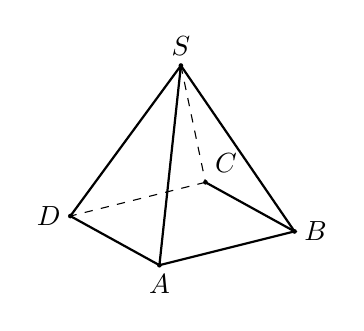
\begin{tikzpicture}[>=stealth,scale=0.78]
  \coordinate (A) at (1.8,0); \coordinate (B) at (4.0,0.55);
  \coordinate (C) at (2.55,1.35); \coordinate (D) at (0.35,0.8);
  \coordinate (S) at (2.15,3.25);
  \draw[thick] (A)--(B)--(C); \draw[dashed] (C)--(D); \draw[thick] (D)--(A);
  \draw[thick] (S)--(A) (S)--(B) (S)--(D);
  \draw[dashed] (S)--(C);
  \fill (S) circle (1.1pt) node[above] {$S$};
  \fill (A) circle (1.1pt) node[below] {$A$};
  \fill (B) circle (1.1pt) node[right] {$B$};
  \fill (C) circle (1.1pt) node[above right] {$C$};
  \fill (D) circle (1.1pt) node[left] {$D$};
\end{tikzpicture}
\end{center}
\nopagebreak[4]
（1） 证明：$SA\perp BC$；

（2） 求直线 $SD$ 与平面 $SAB$ 所成角的大小。

\Needspace{4\baselineskip}
\textbf{解析}

\gksubpart{(1)}

\Needspace{5\baselineskip}
取 $B=(0,0,0),C=(2\sqrt2,0,0)$，由 $\angle ABC=45^\circ$ 可取 $A=(\sqrt2,\sqrt2,0)$。因 $SBC\perp$ 底面，设 $S=(u,0,v)$。由 $SA=SB$ 得 $u=\sqrt2$，于是

\nopagebreak[4]
\[
\overrightarrow{SA}=(0,\sqrt2,-v),\qquad
\overrightarrow{BC}=(2\sqrt2,0,0),
\]

内积为 $0$，故 $SA\perp BC$。

\gksubpart{(2)}

\Needspace{5\baselineskip}
由 $SB^2=3$ 得 $v^2=1$，取 $v=1$。平面 $SAB$ 的一个法向量为 $(-\sqrt2,\sqrt2,2)$，而 $\overrightarrow{SD}=(2\sqrt2,\sqrt2,-1)$，故直线与平面的夹角 $\theta$ 满足

\nopagebreak[4]
\[
\sin\theta=\frac{4}{\sqrt{11}\,2\sqrt2}=\sqrt{\frac2{11}},
\]

即 $\cos\theta=3/\sqrt{11}$。

\gkanswer{答案（1）：见解析版}

\gkanswer{答案（2）：设所成角为 $\theta$，则 $\cos\theta=\dfrac3{\sqrt{11}}$。}

\end{answer}
\begin{answer}
\gksolhead{20}{}

\textbf{题目}：

设函数 $f(x)=2x^3+3ax^2+3bx+8c$ 在 $x=1$ 及 $x=2$ 时取得极值。

（1） 求 $a,b$ 的值；

（2） 若对于任意的 $x\in[0,3]$，都有 $f(x)<c^2$ 成立，求 $c$ 的取值范围。

\Needspace{4\baselineskip}
\textbf{解析}

\gksubpart{(1)}

极值点为 $1,2$，故 $f'(x)=6(x-1)(x-2)$。比较系数得 $a=-3,b=4$。

\gksubpart{(2)}

\Needspace{5\baselineskip}
此时 $f(x)=2x^3-9x^2+12x+8c$，在 $[0,3]$ 上最大值为 $f(3)=8c+9$。条件等价于

\nopagebreak[4]
\[
c^2>8c+9\Longleftrightarrow(c-9)(c+1)>0
\]
，

所以 $c<-1$ 或 $c>9$。

\gkanswer{答案（1）：$a=-3,b=4$。}

\gkanswer{答案（2）：$c\in(-\infty,-1)\cup(9,+\infty)$。}

\end{answer}
\begin{answer}
\gksolhead{21}{}

\textbf{题目}：

设 $\{a_n\}$ 是等差数列，$\{b_n\}$ 是各项都为正数的等比数列，且 $a_1=b_1=1$，$a_3+b_5=21$，$a_5+b_3=13$。

（1） 求 $\{a_n\},\{b_n\}$ 的通项公式；

（2） 求数列 $\left\{\dfrac{a_n}{b_n}\right\}$ 的前 $n$ 项和 $S_n$。

\Needspace{4\baselineskip}
\textbf{解析}

\gksubpart{(1)}

\Needspace{5\baselineskip}
由 $a_n=1+(n-1)d,b_n=q^{n-1}$ 及题设

\nopagebreak[4]
\[
1+2d+q^4=21,\qquad 1+4d+q^2=13
\]
，

令 $r=q^2$，解得 $r=4,d=2$，故 $a_n=2n-1,b_n=2^{n-1}$。

\gksubpart{(2)}

\nopagebreak[4]
\[
\sum_{k=1}^n\frac{a_k}{b_k}
=\sum_{k=1}^n\frac{2k-1}{2^{k-1}}
=6-\frac{2n+3}{2^{n-1}}
\]
。

\gkanswer{答案（1）：$a_n=2n-1$，$b_n=2^{n-1}$。}

\gkanswer{答案（2）：$S_n=6-\dfrac{2n+3}{2^{n-1}}$。}

\end{answer}
\begin{answer}
\gksolhead{22}{}

\textbf{题目}：

已知椭圆 $\dfrac{x^2}{3}+\dfrac{y^2}{2}=1$ 的左、右焦点分别为 $F_1,F_2$，过 $F_1$ 的直线交椭圆于 $B,D$ 两点，过 $F_2$ 的直线交椭圆于 $A,C$ 两点，且 $AC\perp BD$，垂足为 $P$。

（1） 设 $P$ 点的坐标为 $(x_0,y_0)$，证明：$\dfrac{x_0^2}{3}+\dfrac{y_0^2}{2}<1$；

（2） 求四边形 $ABCD$ 的面积的最小值。

\Needspace{4\baselineskip}
\textbf{解析}

\gksubpart{(1)}

\Needspace{5\baselineskip}
两条互相垂直的椭圆弦交于椭圆内部点 $P$，严格凸性给出 $P$ 不在椭圆边界上，因此

\nopagebreak[4]
\[
\frac{x_0^2}{3}+\frac{y_0^2}{2}<1
\]
。

\gksubpart{(2)}

\Needspace{5\baselineskip}
设过右焦点弦 $AC$ 的方向角为 $t$。由直线与椭圆联立，弦长为

\nopagebreak[4]
\[
|AC|=\frac{4\sqrt3}{2\cos^2t+3\sin^2t},
\qquad
|BD|=\frac{4\sqrt3}{2\sin^2t+3\cos^2t}.
\]

\Needspace{5\baselineskip}
因对角线垂直，四边形面积为两对角线乘积的一半，即

\nopagebreak[4]
\[
S=\frac{24}{(3-\cos^2t)(2+\cos^2t)}
\]
。

分母最大值为 $25/4$，故面积最小值为 $96/25$。

\gkanswer{答案（1）：见解析版}

\gkanswer{答案（2）：四边形面积的最小值为 $\dfrac{96}{25}$。}

\end{answer}